\documentclass[preprint,12pt]{elsarticle}

\usepackage{amsmath,amssymb}
\usepackage{graphicx}
\usepackage{booktabs}
\usepackage{longtable}
\usepackage{hyperref}
\usepackage{lineno}
\modulolinenumbers[5]

\journal{Chemometrics and Intelligent Laboratory Systems}

\begin{document}

\begin{frontmatter}

\title{Prior-Guided Spectral Gating Generalizes Across Spectroscopic Modalities: Evidence from Near-Infrared and Raman Spectroscopy}

% *** PLACEHOLDER: author list, order, and affiliations have not been
% confirmed by the corresponding author. Verify before submission. ***
\author[puc]{Clarimar José Coelho\corref{cor1}}
\ead{clarimar@pucgoias.edu.br}
\author[puc]{Guilherme Coelho}
\author[puc]{Angélica Chagas}
\author[puc]{Lilian Carla Carneiro}
\author[unicamp]{Letícia Ritner}
\author[puc]{Marcos Lajovic Carneiro}
\author[ufg]{Arlindo Rodrigues Galvão Filho}
\author[ufpb]{Edvan Cirino da Silva}

\cortext[cor1]{Corresponding author.}
\address[puc]{Pontifícia Universidade Católica de Goiás (PUC Goiás), Goiânia, Brazil}
\address[unicamp]{Universidade Estadual de Campinas (Unicamp), Campinas, Brazil}
\address[ufg]{Universidade Federal de Goiás (UFG), Goiânia, Brazil}
\address[ufpb]{Universidade Federal da Paraíba (UFPB), João Pessoa, Brazil}

\begin{abstract}
Prior-Guided Spectral Gating (PGSG) is a chemometrically-informed spectral attention mechanism that combines a learnable per-band gate, initialized from a literature-derived prior, with an end-to-end regressor. The mechanism has previously been validated exclusively on near-infrared (NIR) spectroscopy, first at small sample sizes and subsequently at scale ($n\approx1{,}448$ mango dry-matter-content spectra, $R^{2}=0.806$ versus $0.568$ for partial least squares, PLS). In this study we test whether the mechanism generalizes, without any architectural modification, to a second spectroscopic modality with markedly different physical structure: Raman spectroscopy. Using a public bioprocess-monitoring benchmark ($n=6{,}472$ spectra, 1,870 Raman-shift variables, glucose concentration as the regression target), we show that the unmodified model --- an independent sigmoid gate per variable feeding a shallow multilayer perceptron, trained end-to-end by backpropagation --- outperforms PLS in Raman as well ($\Delta R^{2}_{\mathrm{PLS}}=+0.025$), reproducing the NIR result at a smaller magnitude ($\Delta R^{2}_{\mathrm{PLS}}=+0.244$ in NIR). We further formalize three quantitative descriptors of learned-gate topology --- entropy, smoothness, and Hoyer sparsity --- and show that Raman gates are more sparse than NIR gates ($0.415$ versus $0.235$--$0.318$, robust to the functional form of the prior) and, once smoothness is correctly normalized by physical band density, smoother in NIR than in Raman, in agreement with raw-spectrum evidence. A literature-informed prior does not improve predictive accuracy over an uninformed initialization in either modality, but substantially increases the reproducibility of the learned gate across random seeds (pairwise Jaccard similarity of the top-weighted decile of bands: $0.90$--$0.94$ versus $0.58$--$0.65$), indicating that the principal value of the prior is interpretive stability rather than accuracy. A finer-grained test correlating local gate structure with literature-reported vibrational linewidths, band by band, did not yield a robust correlation. We report this null result, together with an intermediate finding traced to a specific methodological artifact and a model-identity error that initially reversed our main conclusion, as part of a fully transparent account of the research process.
\end{abstract}

\begin{keyword}
spectral gating \sep interpretable deep learning \sep Raman spectroscopy \sep near-infrared spectroscopy \sep chemometrics \sep cross-modality generalization
\end{keyword}

\end{frontmatter}

\linenumbers

\section{Introduction}
\label{sec:intro}

Prior-Guided Spectral Gating (PGSG) is a chemometrically-informed attention mechanism for spectroscopic regression, in which a learnable gate $g\in(0,1)^{p}$ over $p$ spectral variables is initialized from a literature-derived prior $s$, rather than from the training data, and multiplies the input spectrum before a downstream regressor. The mechanism was originally established on near-infrared (NIR) spectroscopy at small sample sizes \cite{coelho_pgsg0}. A subsequent study revised the architecture --- replacing an earlier formulation, in which a softmax gate weighted a partial-least-squares (PLS) regressor optimized by finite-difference gradients, with an independent sigmoid gate per variable feeding a lightweight multilayer perceptron (MLP) trained end-to-end via automatic differentiation --- and showed that the revised model, hereafter \texttt{PGSGv2Model}, retains a predictive advantage over PLS at substantially larger sample sizes ($n\approx1{,}448$, mango dry-matter content via NIR, $R^{2}=0.806$ versus $0.568$) \cite{coelho_pgsg1,anderson2020}.

Both studies validated PGSG exclusively on NIR, leaving open a basic question about the generality of the mechanism: does prior-guided gating help because of a property specific to NIR spectra, or does it reflect a principle applicable across spectroscopic modalities with different physical structure? NIR spectra are dominated by broad, overlapping overtone and combination bands, in which analyte-relevant signal is typically diluted across many correlated wavelengths \cite{workman2012nir}. Raman spectra, by contrast, exhibit narrow, well-resolved vibrational peaks superimposed on a comparatively flat baseline \cite{smith2019raman}. If the value of prior-guided gating in NIR derives from down-weighting broad, uninformative regions in favor of a chemically relevant subset, the mechanism might contribute comparatively little in a modality where informative peaks are already narrow and readily isolated by the regressor.

We test this directly by applying the unmodified \texttt{PGSGv2Model} architecture to a Raman regression task and by formalizing quantitative descriptors of learned-gate topology --- entropy, smoothness, and sparsity --- to characterize \emph{how}, not merely \emph{whether}, gate structure differs between the two modalities. We evaluate five falsifiable hypotheses (Section~\ref{sec:hypotheses}) end to end on public NIR and Raman benchmarks and, in the interest of transparency, document a model-identity error made during execution of this study that initially produced results opposite to those reported here for the central hypothesis (Section~\ref{sec:model-identity}).

\section{Scope}
\label{sec:scope}

An early planning stage of this work considered simultaneous generalization to four modalities: NIR, Raman, mid-infrared (MIR), and mass spectrometry (MS). This scope was narrowed to two modalities for two reasons. First, validating across four modalities within a single study risks the inverse of a problem already identified and corrected in prior work \cite{coelho_pgsg1}: an empirical scope exceeding what can be executed and tested with rigor. Second, the physical argument motivating spectral gating --- correlation between adjacent positions along a continuous spectral axis --- does not hold for MS, whose signals are discrete mass-to-charge values without an analogous local neighborhood structure; including MS without adapting the gating operator itself would constitute a weak extension. MIR and MS therefore remain outside the empirical scope of this study.

\section{Hypotheses}
\label{sec:hypotheses}

\begin{description}
\item[H1 (generalization without architectural change).] \texttt{PGSGv2Model}, applied to Raman data without architectural modification (only reconfiguration of the initialization prior), outperforms PLS, reproducing the NIR result qualitatively ($\Delta R^{2}_{\mathrm{PLS}}>0$).
\item[H2 (differential sparsity).] The gate learned on Raman data is significantly more sparse (Hoyer index) than the gate learned on NIR data, reflecting the narrow-peak structure of Raman scattering relative to the broad, overlapping overtone and combination bands of NIR.
\item[H3 (differential smoothness).] The gate learned on NIR data is significantly smoother (normalized total variation) than on Raman.
\item[H4 (value of a physically motivated prior).] Initializing the gate from literature-derived vibrational assignments, rather than from an uninformed initialization, yields predictive performance that is equal to or better, and gate stability across training seeds that is greater, in both modalities.
\item[H5 (structure--physics correlation).] The entropy and smoothness of the learned gate correlate with the known spectral bandwidth of the vibrational transitions relevant to the target analyte, within a given modality.
\end{description}

\section{Materials and Methods}
\label{sec:methods}

\subsection{Datasets}
\label{sec:datasets}

The NIR branch reuses the Mango DMC v3 dataset (dry-matter content, \%; $n=1{,}448$ in Season~4, the invariant test season used throughout) \cite{anderson2020} and the associated literature-derived prior from the prior study \cite{coelho_pgsg1,saranwong2004}. The Raman branch uses \texttt{bioprocess\_substrates} \cite{lange2026}, a bioprocess-monitoring benchmark accessed through the RamanBench collection \cite{koddenbrock2026}, with glucose concentration as the regression target. Of 6,960 spectra in the source dataset, 6,472 carry a valid glucose label and were retained ($p=1{,}870$ Raman-shift variables spanning 390.6--3384.7~cm$^{-1}$). Table~\ref{tab:datasets} summarizes both branches.

This dataset was selected, among 58 regression datasets available in RamanBench, on the basis of three criteria: a real (non-simulated) measurement, a single chemically interpretable target, and a sample size of the same order of magnitude as the NIR branch ($n\approx12{,}000$). The latter criterion avoids the small-sample regime that characterizes most publicly available Raman regression datasets and that would otherwise confound modality with sample size; alternative candidates considered and not selected for this reason include organic-acid concentration datasets from inline process monitoring \cite{echtermeyer2021}, which are real measurements but of substantially smaller sample size.

\begin{table}[htbp]
\centering
\caption{Summary of the two experimental branches.}
\label{tab:datasets}
\begin{tabular}{lll}
\toprule
& NIR & Raman \\
\midrule
Dataset & Mango DMC v3, Season 4 & \texttt{bioprocess\_substrates} \\
Target & Dry matter content (\%) & Glucose concentration \\
$n$ (valid samples) & 1,448 & 6,472 \\
$p$ (variables, after cleaning) & 281 & 1,870 \\
Spectral range & 285--1200~nm & 390.6--3384.7~cm$^{-1}$ \\
Train/test split & 80/20, stratified & 80/20, stratified \\
\bottomrule
\end{tabular}
\end{table}

\subsection{Preprocessing}

The NIR branch reuses the existing preprocessing operator unchanged: removal of instrument-edge bands with systematically zero values, followed by standard normal variate (SNV) normalization \cite{barnes1989snv}. For Raman, the preprocessing chain --- extended, not rewritten, from the same software contract --- comprises: (i) cosmic-ray removal via a modified Z-score computed on the first derivative \cite{whitaker2018}, restricted to contiguous runs of at most three points so that the steep edges of genuine narrow Raman peaks are not misidentified as spikes; (ii) baseline correction by asymmetric least squares \cite{eilers2005}, removing the fluorescence background characteristic of Raman measurements; and (iii) SNV normalization.

\subsection{Architecture}

Both branches use the identical \texttt{PGSGv2Model}: an independent sigmoid gate per variable, $g_i=\sigma(\theta_i)$, multiplying the input spectrum elementwise, followed by a shallow MLP (one hidden layer, 32 units, ReLU activation, dropout), trained end-to-end by backpropagation (Adam optimizer \cite{kingma2015adam}, weight decay $10^{-4}$, early stopping on a held-out validation split). The gate parameters $\theta$ are initialized from a prior $s\in(0,1)^{p}$ through the logit transform, $\theta_0=\mathrm{logit}(s)$, so that $g$ starts exactly at $s$. No architectural component differs between modalities; this identity constitutes the condition under which H1 is tested.

\subsection{Priors}

For NIR, the prior is a fixed step function over three literature-derived spectral regions relevant to dry matter content --- 680--700~nm (chlorophyll), 900--1000~nm (second C--H overtone), and 1100--1200~nm (first C--H overtone) \cite{saranwong2004} --- independent of the training data. For Raman, the prior is a mixture of Gaussian components centered on literature-reported glucose Raman bands, at two confidence tiers: three primary bands (911, 1060, and 1125~cm$^{-1}$) supported by multiple independent sources \cite{lyu2012,kang2020}, and a secondary set of sixteen bands specific to bioprocess culture-medium monitoring, from a single source \cite{uspatent2024}. In both modalities the prior is constructed solely from published band assignments, never from the experiment's own training data --- a design choice made to avoid the circularity that would result from deriving the prior and the target from the same sample.

\subsection{Gate topology descriptors}
\label{sec:topology}

Let $g\in(0,1)^{p}$ denote the learned gate. Because the gate is an independent sigmoid per variable, $\sum_i g_i \neq 1$ in general, unlike a softmax gate; entropy is therefore computed on the normalized gate. The three descriptors are defined as
\begin{align}
H(g) &= -\sum_{i=1}^{p} \hat g_i \log \hat g_i, \qquad \hat g_i = \frac{g_i}{\sum_j g_j} \label{eq:entropy}\\
\mathrm{TV}(g) &= \frac{1}{p-1}\sum_{i=1}^{p-1} |g_i - g_{i+1}| \label{eq:tv}\\
S(g) &= \frac{\sqrt{p}-\|g\|_1/\|g\|_2}{\sqrt{p}-1} \in [0,1] \label{eq:hoyer}
\end{align}
where Eq.~\eqref{eq:hoyer} is the sparsity index of \cite{hoyer2004}; $S(g)=0$ corresponds to a uniformly dense gate and $S(g)=1$ to a one-hot gate. Cross-modality comparison of $\mathrm{TV}(g)$ requires an additional normalization by physical band density, described in Section~\ref{sec:results-h2h3}.

\subsection{Experimental protocol}

All experiments use a within-dataset (intra-domain) protocol: a fixed, disjoint test split (80/20, stratified where applicable) within each dataset, avoiding cross-domain comparisons that prior work found to substantially degrade performance --- a cross-season protocol on the NIR dataset reduced PLS $R^{2}$ to approximately $0.06$ \cite{coelho_pgsg1}.

\subsection{Additional baselines}
\label{sec:baselines}

Beyond PLS, the broader research program plans to include ABRN \cite{huang2019}, an attention-based residual network without prior guidance; SpecFuseNet \cite{kabiso2025}, a residual autoencoder with channel attention; and sparse linear baselines (Elastic Net, sparse PLS). These additional comparisons address predictive performance only, not gate topology, and do not alter the scope of H1--H5.

\section{A note on model identity}
\label{sec:model-identity}

During execution of this study, an earlier and never-published PGSG implementation --- a softmax gate over a PLS regressor optimized by finite-difference gradients --- was inadvertently substituted for \texttt{PGSGv2Model} in an initial round of Raman experiments. This earlier implementation had never been used to produce any previously published result. Under it, gate training on Raman terminated at the very first epoch, with no improvement over the prior-initialized gate at any subsequent step, and $\Delta R^{2}_{\mathrm{PLS}}\approx0$, leading to an initial and incorrect conclusion that H1 was not supported, tentatively attributed to gate over-parameterization. Once the discrepancy was identified and the correct architecture substituted, the opposite result was obtained (Section~\ref{sec:results-h1}). We report this explicitly, together with the diagnostic evidence for both versions, as part of a transparent scientific record; the associated code, data, and commit history are publicly available (Section~\ref{sec:availability}).

\section{Results}
\label{sec:results}

\subsection{H1: generalization without architectural change}
\label{sec:results-h1}

\texttt{PGSGv2Model}, applied to the Raman dataset without architectural modification, outperforms PLS (Table~\ref{tab:h1}, Fig.~\ref{fig:h1}): $R^{2}_{\mathrm{PLS}}=0.9044$, $R^{2}_{\mathrm{PGSGv2}}=0.9290$, $\Delta R^{2}_{\mathrm{PLS}}=+0.0246$. Under the identical protocol, the NIR branch yields $R^{2}_{\mathrm{PLS}}=0.5684$, $R^{2}_{\mathrm{PGSGv2}}=0.8128$, $\Delta R^{2}_{\mathrm{PLS}}=+0.2444$. Both results reflect genuine gate training rather than a frozen initialization: the best validation epoch occurs at epoch~79 (of up to 500, patience 30) in Raman and epoch~469 in NIR, and the correlation between the learned gate and its initializing prior falls to $\rho=0.978$ (Raman) and $\rho=0.998$ (NIR) --- a measurable, if modest, departure from initialization in both cases. \textbf{H1 is supported.}

\begin{table}[htbp]
\centering
\caption{H1: predictive performance, PLS versus \texttt{PGSGv2Model}.}
\label{tab:h1}
\begin{tabular}{lccc}
\toprule
Modality & $R^{2}_{\mathrm{PLS}}$ & $R^{2}_{\mathrm{PGSGv2}}$ & $\Delta R^{2}_{\mathrm{PLS}}$ \\
\midrule
NIR & 0.5684 & 0.8128 & $+0.2444$ \\
Raman & 0.9044 & 0.9290 & $+0.0246$ \\
\bottomrule
\end{tabular}
\end{table}

\begin{figure}[htbp]
\centering
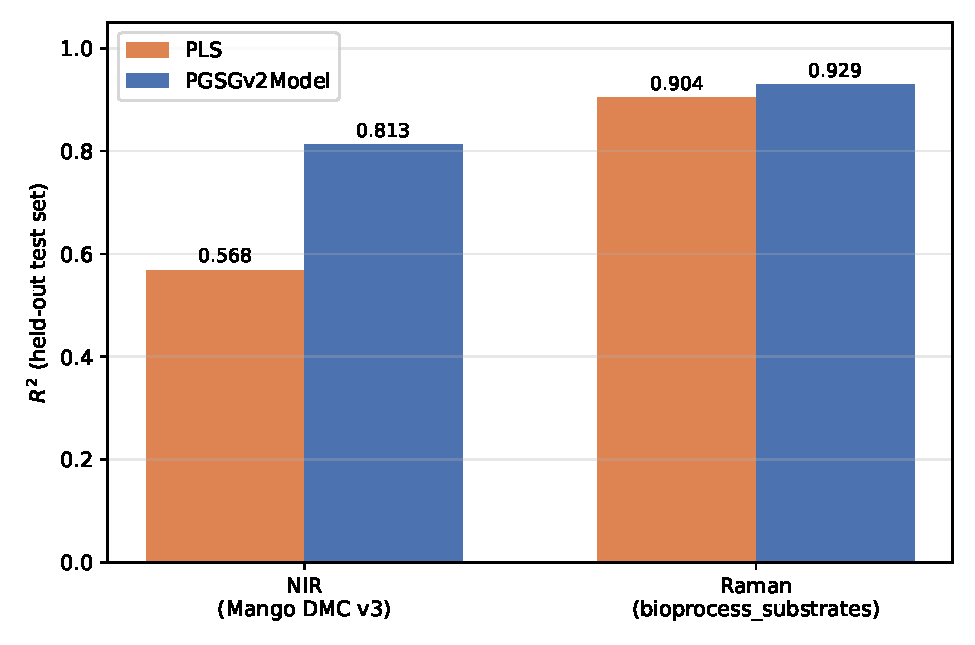
\includegraphics[width=0.7\linewidth]{h1_performance.pdf}
\caption{Predictive performance ($R^{2}$, held-out test set) of PLS and \texttt{PGSGv2Model} in each modality.}
\label{fig:h1}
\end{figure}

\subsection{H2 and H3: gate topology across modalities}
\label{sec:results-h2h3}

\textbf{H2 (sparsity) is supported and robust to the functional form of the prior.} With each modality's original prior form, Hoyer sparsity is $S_{\mathrm{NIR}}=0.3176$ versus $S_{\mathrm{Raman}}=0.4150$ (Fig.~\ref{fig:h2h3}a). To rule out an encoding artifact --- the NIR prior is a step function, whereas the Raman prior is a Gaussian mixture --- the NIR prior was recoded as Gaussian bumps at the same literature centers and relative weights, matching the Raman encoding. The difference persists and widens ($S_{\mathrm{NIR}}=0.2345$ versus $S_{\mathrm{Raman}}=0.4150$), indicating that the effect is not attributable to prior-encoding style.

\textbf{H3 (smoothness) requires a methodological correction.} A first comparison of $\mathrm{TV}(g)$ by raw variable index yielded the result opposite to that predicted: $\mathrm{TV}_{\mathrm{NIR}}=0.0167 > \mathrm{TV}_{\mathrm{Raman}}=0.0076$ (Fig.~\ref{fig:h2h3}b). This reversal persisted under the Gaussian-prior ablation and is therefore not a prior-encoding artifact. Its cause is a difference in spectral sampling density: the NIR axis ($p=281$ variables over $\approx26{,}755$~cm$^{-1}$, $\approx95$~cm$^{-1}$ per variable) is approximately sixty times sparser, in wavenumber terms, than the Raman axis ($p=1{,}870$ variables over $\approx2{,}995$~cm$^{-1}$, $\approx1.6$~cm$^{-1}$ per variable). Total variation computed per variable index conflates the number of variables separating two informative regions with the smoothness of the transition per unit of physical spectrum, and is therefore an unsuitable metric for comparison across modalities with such disparate variable densities.

Recomputing smoothness per unit of physical bandwidth --- converting the NIR axis from nanometers to wavenumbers via $\tilde\nu=10^{7}/\lambda$ --- reverses the direction, now matching the hypothesis: $\mathrm{TV}_{\mathrm{physical,NIR}}=3.69\times10^{-4} \ll \mathrm{TV}_{\mathrm{physical,Raman}}=3.80\times10^{-3}$ (Fig.~\ref{fig:h2h3}c). This is corroborated by an independent check, unrelated to any gate or prior: the raw preprocessed spectrum is approximately $2.3$-fold rougher (point-to-point variation) in Raman than in NIR ($0.2156$ versus $0.0926$). Two independent measures agree once the density confound is removed. \textbf{H3 is supported}, provided smoothness is measured per unit of physical spectrum rather than per raw variable index; we note that the raw-index comparison is unreliable for cross-modality use in general and should be avoided in future work of this kind.

\begin{figure}[htbp]
\centering

\includegraphics[width=\linewidth]{h2h3_topology.pdf}
\caption{Gate topology across modalities. (a) Hoyer sparsity: Raman more sparse than NIR under both prior encodings. (b) Smoothness by raw variable index: a misleading comparison, dominated by the difference in spectral sampling density between modalities. (c) Smoothness normalized by physical unit (cm$^{-1}$): the correct comparison, in agreement with raw-spectrum roughness.}
\label{fig:h2h3}
\end{figure}

\subsection{H4: value of a physically motivated prior}
\label{sec:results-h4}

Across ten training seeds per condition, predictive performance is statistically equivalent between literature-informed and uninformed (zero) initialization in both modalities (Table~\ref{tab:h4}): NIR, $R^{2}_{\mathrm{lit}}=0.7933\pm0.0080$ versus $R^{2}_{\mathrm{rand}}=0.7983\pm0.0077$; Raman, $R^{2}_{\mathrm{lit}}=0.9302\pm0.0015$ versus $R^{2}_{\mathrm{rand}}=0.9310\pm0.0014$. Gate stability across seeds, in contrast, differs sharply and consistently in favor of the informed prior (Fig.~\ref{fig:h4}): pairwise gate correlation $\rho=0.9995$ (NIR, literature prior) versus $0.8653$ (NIR, uninformed), and $0.9976$ (Raman, literature prior) versus $0.8931$ (Raman, uninformed); pairwise Jaccard similarity of the top-weighted decile of variables, $0.9418$ (NIR, literature prior) versus $0.6002$ (NIR, uninformed), and $0.9011$ (Raman, literature prior) versus $0.6545$ (Raman, uninformed).

\begin{table}[htbp]
\centering
\caption{H4: performance and gate stability, literature prior versus uninformed initialization (10 seeds).}
\label{tab:h4}
\begin{tabular}{lcccc}
\toprule
& \multicolumn{2}{c}{NIR} & \multicolumn{2}{c}{Raman} \\
& Literature prior & Uninformed & Literature prior & Uninformed \\
\midrule
$R^{2}$ (mean $\pm$ SD) & $0.7933\pm0.0080$ & $0.7983\pm0.0077$ & $0.9302\pm0.0015$ & $0.9310\pm0.0014$ \\
$\rho$ (pairwise) & 0.9995 & 0.8653 & 0.9976 & 0.8931 \\
Jaccard (pairwise) & 0.9418 & 0.6002 & 0.9011 & 0.6545 \\
\bottomrule
\end{tabular}
\end{table}

\begin{figure}[htbp]
\centering

\includegraphics[width=\linewidth]{h4_prior_ablation.pdf}
\caption{H4: literature-informed prior versus uninformed initialization, 10 training seeds. (a) Predictive performance is statistically equivalent. (b) Gate stability across seeds is substantially higher with the literature-informed prior, in both modalities.}
\label{fig:h4}
\end{figure}

\textbf{H4 is supported for gate stability}; the accuracy component of the hypothesis (``equal to or better than'') holds only in the weak sense of statistical equivalence, not superiority, in either modality.

\subsection{H5: structure--physics correlation}
\label{sec:results-h5}

H5, as originally stated across modalities, is not testable as a statistical correlation with only two modalities ($n=2$). We reformulate it as a within-modality, band-by-band test in Raman, correlating literature-reported linewidths for twenty glucose Raman bands \cite{uspatent2024} against three descriptors extracted locally around each band from the trained gate, within an adaptive window capped at 45\% of the distance to the nearest neighboring literature band, to avoid cross-contamination between closely spaced bands such as the 1060/1073~cm$^{-1}$ pair. NIR is excluded from this quantitative test: it has only three literature bands, and its prior already encodes their exact literature widths by construction, which would render any correlation circular.

None of the three local descriptors yields a robust, correctly signed correlation (Fig.~\ref{fig:h5}, $n=20$): local gate full width at half maximum, $r=+0.254$ ($p=0.279$); local smoothness, $r=+0.048$ ($p=0.840$); local entropy, computed raw, $r=+0.407$ ($p=0.075$, marginal, correct direction), and normalized by window size ($\log n$), $r=-0.636$ ($p=0.003$, significant but in the direction opposite to that predicted). Diagnosis traced the entropy instability to the adaptive window itself: narrow windows, required near closely spaced bands, sample predominantly the flat top of a Gaussian bump, mechanically inflating normalized entropy toward its ceiling regardless of true local structure, whereas wider windows capture more of the true rise and fall, pulling the metric down. A synthetic control with a known, built-in correlation (gate bump width proportional to literature width by construction) confirmed that the extraction method recovers the expected correlation when it exists ($r=0.73$, $0.57$, and $-0.86$ for the three descriptors, all $p<0.01$), indicating that the null result on real data is informative rather than a failure of the extraction procedure. \textbf{H5 is not supported.} Further refinement of the windowing scheme was not pursued, to avoid the risk of adjusting a method until it yields the expected significance.

\begin{figure}[htbp]
\centering
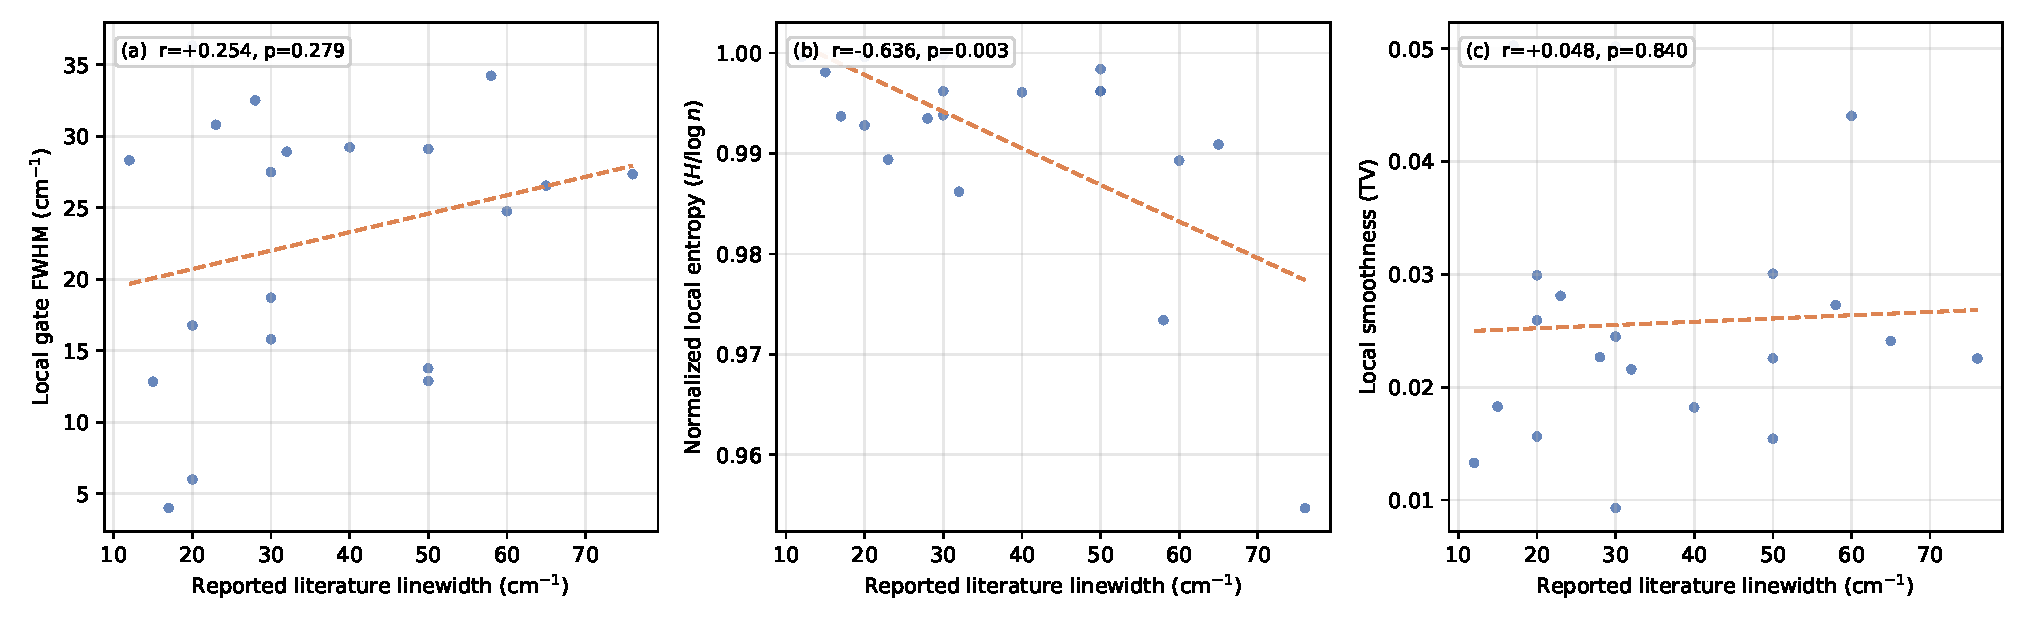
\includegraphics[width=\linewidth]{h5_correlation.pdf}
\caption{H5: literature-reported linewidth versus local gate descriptors, Raman, $n=20$ bands. Dashed lines show ordinary least-squares fits. None of the three descriptors shows a robust, correctly signed correlation.}
\label{fig:h5}
\end{figure}

\section{Discussion}
\label{sec:discussion}

Table~\ref{tab:summary} summarizes the outcome of the five hypotheses.

\begin{table}[htbp]
\centering
\caption{Summary of hypothesis tests.}
\label{tab:summary}
\begin{tabular}{p{1cm}p{4.6cm}p{7.4cm}}
\toprule
Hyp. & Outcome & Key evidence \\
\midrule
H1 & Supported & $\Delta R^{2}_{\mathrm{PLS}}=+0.0246$ (Raman), $+0.2444$ (NIR); identical architecture \\
H2 & Supported, robust & Hoyer sparsity: Raman $0.415$ > NIR $0.235$--$0.318$ (two prior encodings) \\
H3 & Supported, with correction & Smoothness per cm$^{-1}$: NIR $3.69\times10^{-4} \ll$ Raman $3.80\times10^{-3}$; consistent with raw-spectrum roughness \\
H4 & Supported (stability); performance equivalent & Pairwise gate $\rho$: $0.998$--$0.9995$ (prior) versus $0.86$--$0.89$ (uninformed), both modalities \\
H5 & Not supported & No local descriptor correlates robustly with real per-band linewidth ($n=20$, Raman) \\
\bottomrule
\end{tabular}
\end{table}

Taken together, the five results suggest a coherent mechanistic account. In both modalities the learned gate remains close to its initializing prior ($\rho\geq0.98$), indicating that the model's advantage over PLS derives substantially from weighting the spectrum by chemically informed prior knowledge before regression rather than from extensive gradient-driven refinement of the gate. This reading also explains the difference in magnitude between the two modalities in H1: NIR spectra dilute analyte-relevant signal across many broad, overlapping, low-sparsity variables (H2, H3), so down-weighting uninformative regions substantially improves an otherwise weak PLS baseline ($R^{2}$ increasing from $0.568$ to $0.813$); Raman spectra are already sparse and narrow, so PLS applied to the raw spectrum already isolates the relevant signal ($R^{2}=0.904$), leaving comparatively little room for the prior weighting to add value ($R^{2}=0.929$).

H4 refines this picture further: the value of the prior lies not in predictive accuracy --- statistically indistinguishable with or without it --- but in the reproducibility of the learned attention pattern across independent training runs. A gate that points to different variables on every run is not a trustworthy explanation, even when its predictions are accurate; a physically motivated prior appears to function principally as an anchor for interpretability rather than as a performance lever.

H5, the single negative result, probes a stronger and more granular claim than H2/H3: not merely that aggregate gate topology differs between modalities in a manner consistent with physics (established by H2/H3), but that local gate structure, band by band, tracks the specific linewidth of each vibrational transition. With twenty Raman bands, none of the three descriptors tested produced a robust, replicable correlation, and the entropy descriptor proved unstable enough to reverse sign under a defensible alternative normalization. We interpret this as a resolution limit of the current descriptors rather than evidence that the gate is physically uninformative at a local level: gate topology appears to capture between-modality structural differences without necessarily resolving fine within-modality variation at the level of individual bands, at least with the windowing scheme used here.

\subsection{Limitations}

Three limitations apply across the study. First, the research process included a consequential correction: an unpublished, superseded PGSG implementation was inadvertently used for an initial round of Raman experiments, producing a conclusion opposite to the one that holds under the correct architecture (Section~\ref{sec:model-identity}); this is documented in full in the public repository. Second, cross-modality topology comparisons require careful normalization by physical band density (Section~\ref{sec:results-h2h3}); future extensions of this line of work, including within the same research program, should adopt the same caution. Third, H4 was evaluated with ten training seeds per condition; a larger number would strengthen the stability estimate, although the observed effect is already large and consistent across both modalities.

\section{Conclusion}

Prior-Guided Spectral Gating generalizes, without architectural modification, from near-infrared to Raman spectroscopy, and its learned gate exhibits topological differences between the two modalities that are consistent with their underlying physical structure once compared on a physically meaningful basis. The magnitude of the predictive advantage, however, depends on how redundant or diluted the analyte-relevant signal already is in a given modality: substantial in NIR, modest in Raman. The principal contribution of a literature-informed prior appears to be the reproducibility of the resulting interpretation across training runs rather than raw accuracy. A finer, band-level test of structure--physics correspondence did not succeed with the descriptors used here, a negative result reported alongside the positive ones. These findings inform subsequent stages of the broader research program (multi-target regression, systematic hyperparameter optimization, uncertainty quantification), for which the expected benefit of spectral gating should be assessed on a case-by-case basis rather than assumed uniform across modalities and targets.

\section*{Data and code availability}
\label{sec:availability}
All code, experiment scripts, saved model outputs, and the commit history documenting the model-identity correction described in Section~\ref{sec:model-identity} are available at \url{https://github.com/clarimar/pgsg2-nir-raman-gating}.

\section*{Acknowledgments}
% *** PLACEHOLDER: to be completed with funding/acknowledgment information. ***

\bibliographystyle{elsarticle-num}
\bibliography{pgsg_2_refs}

\end{document}
